%!TEX root = ../diffusion_paper.tex
\section{Introduction} % (fold)
\label{sec:introduction}
  \IEEEPARstart{A}{ll} 3D histology reconstruction methods are based on the acquisition of individual 2D histology images, whether from scans of the un-cut surface of the embedded tissue (so-called block face imaging) \cite{Sands2005,Sands2006,Rutherford2012}, or as sections \cite{Burton2006,Plank2009}. In the former case, 2D images are intrinsically registered, and so no alignment is necessary. In the latter case, images are brought into alignment either through registration amongst themselves, or to a coherent reference volume. It will be seen that the most recent methods draw together the advantages of both techniques.
  
  In 2002, Hooks et al. \cite{Hooks2002} sectioned a 0.8 x 0.8 x 3.7mm transmural segment of rat left ventricle and recorded an intrinsically registered volume image of cubic-1.56$\mu$m resolution using confocal microscopy. The resulting volume images were more detailed than any that had been seen before. Using similar techniques in 2012, Rutherford et al. \cite{Rutherford2012} produced a 5.6mm$^3$ volume surrounding a rat anterior left ventricular infarct, with cubic-1$\mu$m resolution. Unfortunately, this approach cannot resolve tissue sections much larger than the samples presented, and certainly not an entire heart.
  
  It is well documented in the literature that the asymmetrical curvature of an object cannot be recovered solely from a set of two dimensional sections. This issue is known as the `banana problem' \cite{Malandain2004,Lyon2012} or the `z-shift effect' \cite{Yushkevich2006}. Even so, substantial literature is published attempting to reconstruct volumes in the absence of a target geometry \cite{Chakravarty2006,Schmitt2006,Cifor2009,Cifor2011}.
  
  Registering slices to a reference volume circumvents the banana problem. Burton et al. \cite{Burton2006} paved the way for this conjunction by providing MRI rabbit cardiac images of 26.4 x 26.4 x 24.4$\mu$m voxel size with 1.1 x 1.1 x 10$\mu$m histology stacks of the same hearts. They exhibited an initial attempt at slice alignment, guided by the MRI data. First, the difference between adjacent slices was minimised by applying rigid 2D transformations to each slice. Next, they applied a partial differential equation-based approach, solved using a pyramidal and geometric multigrid scheme. While this approach is often used to correct distortion in histological images \cite{Keeling2005}, and is indeed capable of correcting major misalignments, it has an important drawback: by aligning adjacent slices they reduce inter-slice differences that might be fundamental in the description of heart anatomy.
  
  Since then, an automated pipeline has been developed, applying iterative 2D and 3D optimised deformations to register the stacks into the MRI geometry \cite{Mansoori2007}. Histology slices were stacked together into a volume and a rigid 3D transform was optimised to get an initial rough alignment with the MRI volume. Each histology slice was then rigidly registered in its 2D plane with the corresponding MRI slice. Iterations of 3D and 2D registrations are performed until the optimal rigid registration between the two volumes is obtained. In the last stage, non-rigid histology to MRI slice registration was performed using the Demons algorithm \cite{Thirion1995}. Histogram matching was applied as a preliminary step to ensure equal intensities between the two images, as required by the Demons algorithm. Despite some success with this procedure, the slices are ultimately registered to 2D MRI image that does not correspond to the histology, and the unconstrained non-rigid registration that was employed in the final stage led to unrealistic tissue distortions. These problems notwithstanding, the direct registration of histology to MRI is the best way to move towards global shape correctness if no other reference data is available, and is still a common procedure \cite{Alic2011,Osechinskiy2011,Kimm2012}.
  
  Some of the simplest reference-based registration methods rely on manual feature selection or expert hand-drawn atlases. Jagular et al. \cite{Jagalur2007} register thousands of mouse brain histological gene-expression images to expert atlases using automatically selected landmarks. An expert manual approach, whilst appropriate for a quick and approximate result from a small number of data, does not scale, is not repeatable and is prone to human bias.
  
  Block face images, taken from the surface of the fixated tissue volume before sectioning, provide an intrinsically coherent and precisely corresponding set of reference images. Although suitable for low-resolution alignment  \cite{Palm2010}, the reference images are very different in appearance to the histology, with a much lower spatial resolution, hindering accurate alignment. Even very small imperfections in the final mappings introduces jaggedness that renders volumetric microstructure almost imperceptible. Algorithms have been proposed to smooth out this noise through the more precise and reliable coregistration of adjacent slices, in both a sequential \cite{Yushkevich2006,Chakravarty2008} and simultaneous \cite{Feuerstein2011} manner. However, these methods are highly parameterised, often involving registrations at a number of scales, using only a subset of the image information available, and are often based on essentially subjective segmentations, rather than purely original images. Furthermore, only the nearest two neighbouring slices are used to dampen transformational noise, and therefore only the very highest frequency of noise can ever be reduced. Most recently, high-resolution reference images have been provided through the use of two-photon tomography and microtomy \cite{Huang2009,Ragan2012}.
  
  Yushkevich et al. \cite{Yushkevich2006,Adler2012} attempt to correct for the banana effect in a serially registered mouse brain histological volume. They first perform a rigid-body banana registration to approximate the dimensions of a full cardiac volume. Clearly, if a transform less constrained than rigid-body were used, then each slice would resemble the size and, depending on the constraint of the transform, the shape of the first reference slice. A prism-like volume would result, entirely unrelated to the true geometry of the heart. They obtain resampled 2D MRI images corresponding to each section via a rigid 3D registration of the MRI to the z-shifted histology. The volume produced from registering each section to these MRI images is jagged, and so the transformation parameters are Gaussian smoothed to recover some of the continuity of the serial volume. This approach goes a long way to combining the global fidelity of anchoring to a reference volume and the local smoothness of adjacent slice registration. Yet smoothness is limited by the level of success of the individual inter-slice registrations; any error or discontinuity in the serial volume will be transduced directly into the final result. In particular, any differential deformation of adjacent slices during sectioning, either affine or curved, could not be resolved by the rigid-body banana registration, and would manifest as disjoints through the tissue in the z-direction. Moreover, they themselves concede that the method entails a great deal of empirical parameterisation and manual intervention, from the slice segmentation, to the graph edge weighting of the adjacent slice selection, to the width of the Gaussian smoothing of the histology-to-MRI transform parameters.
  
  No mention of non-rigid transforms is mentioned in the Yushkevich implementation. But conceivably, non-rigid interslice registrations could be integrated into the pipeline once the MRI correspondence planes had been established, initialised from the terminus of the rigid registrations. In this case, one would be faced with two disagreeable alternatives. On the one hand, a direct registration could be performed from each slice in the cylindrical, non-rigid banana volume to the reference volume. In this case, most of the slices would be so distant in size, shape and position from alignment with the reference slice as to preclude consistent, successful registration. A better solution would apply the Gaussian smoothing to the transforms from the non-rigid, prism-like banana volume to the reference volume. These transforms could be computed by composing the inverse of the transforms from the rigid banana volume to the non-rigid volume with the transforms from the rigid banana volume to the reference volume. Volumes would certainly be smoother than with the rigid smoothing, as adjacent non-rigid differences have been relaxed. Yet inevitable occasional errors and inaccuracies in alignment would still be present, as slices are only given one algorithmic run to align, and it is implausible that the freedoms inherent in the transform of choice exactly correspond to the distortions undergone by the tissue sections.
  
  Chakravarty et al. \cite{Chakravarty2008} first rigidly align sections of whole mouse brain to an associated block face set, then apply a deformation field transformation to each slice, calculated as the mean of the parameters from defomation fields registering it to the two neighbouring slices. While this may go some way to reducing noise from the block face registrations, the maximum distance of information transfer is one slice, and so only the maximum distortion frequency will be damped.
  
  Techniques have been developed to combine monomodal adjacent slice and multimodal reference registrations simultaneously. Palm et al. \cite{Palm2008} expound a `weighted multi-image mutual information metric', optimising the sum of scaled contributions from both cost functions, and Feuerstein et al. \cite{Feuerstein2011} combine two potential energy functions in a Markov random field model to reconstruct a rat kidney. Not only do these methods require extraneous parameterisation and tuning, but in practice, the superposed cost function will form several distinct local minima; rather than reaching an averaged compromise between the reference images, the optimisation will arrive close to one preferred of several single-image minima, depending on the relative weightings and the transform initialisation.
  
  Atlases of both histology and MRI have been constructed by averaging histological volumes \cite{Li2009}, which were registered based on the approaches taken by \cite{Malandain2004,Yushkevich2006}. Having segmented mouse brain sections, their centres of mass were aligned and a rigid body registration was performed between adjacent slices. The banana effect was mitigated by a 3D registration to MRI, a slice-wise alignment of histological centres of mass to their MRI cross-section equivalent, and a final 3D non-rigid registration. Whilst perhaps appropriate for such low resolution data as presented, these methods are heuristic at best, and introduce several artificial sources of distortion.
  
  Finally, \cite{Arganda-Carreras2010} offer an interesting and robust approach to combining monomodal and multimodal alignments, using consistent b-spline-based elastic registrations. Multiple iterations of triple-wise registrations gradually share information in the z-direction and result in smoothing through a spectrum of scales. However, the choice of simultaneous registration leads to the same problem of multiple local minima faced by \cite{Palm2008,Feuerstein2011}.
  
  % \hfill mds
  %  
  % \hfill January 11, 2007
  % 
  
  % needed in second column of first page if using \IEEEpubid
  %\IEEEpubidadjcol

  % An example of a double column floating figure using two subfigures.
  % (The subfig.sty package must be loaded for this to work.)
  % The subfigure \label commands are set within each subfloat command, the
  % \label for the overall figure must come after \caption.
  % \hfil must be used as a separator to get equal spacing.
  %
  %\begin{figure*}[!t]
  %\centerline{\subfloat[Case I]\includegraphics[width=2.5in]{subfigcase1}%
  %\label{fig_first_case}}
  %\hfil
  %\subfloat[Case II]{\includegraphics[width=2.5in]{subfigcase2}%
  %\label{fig_second_case}}}
  %\caption{Simulation results}
  %\label{fig_sim}
  %\end{figure*}
  %
  % Note that often IEEE papers with subfigures do not employ subfigure
  % captions (using the optional argument to \subfloat), but instead will
  % reference/describe all of them (a), (b), etc., within the main caption.
  
  \begin{figure}[!t]
    \centering
    \subfloat[]{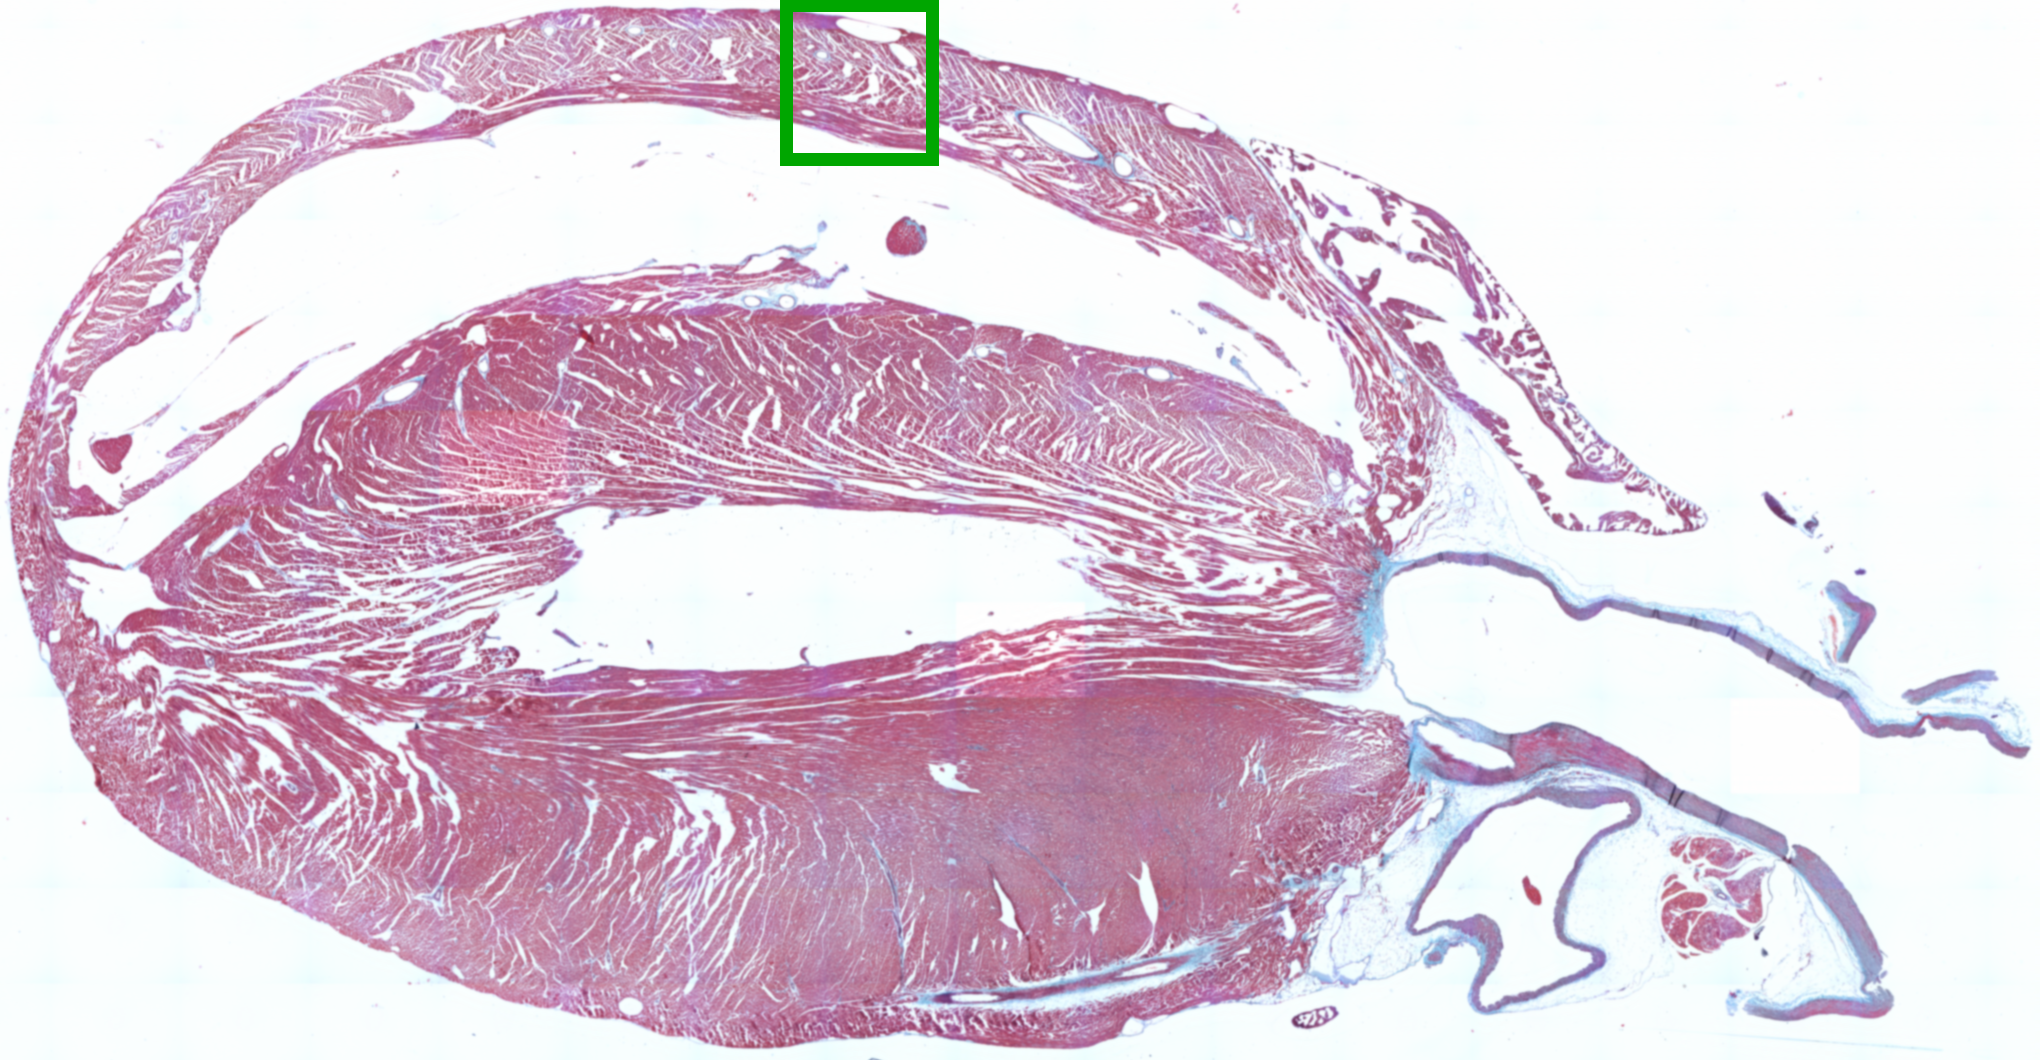
\includegraphics[width=1.7in]{1_introduction/Figs/HiRes_downsamples_8_0582}}
    \subfloat[]{\includegraphics[width=1.7in]{1_introduction/Figs/LoRes_rgb_downsamples_1_0582}}\\
    \subfloat[]{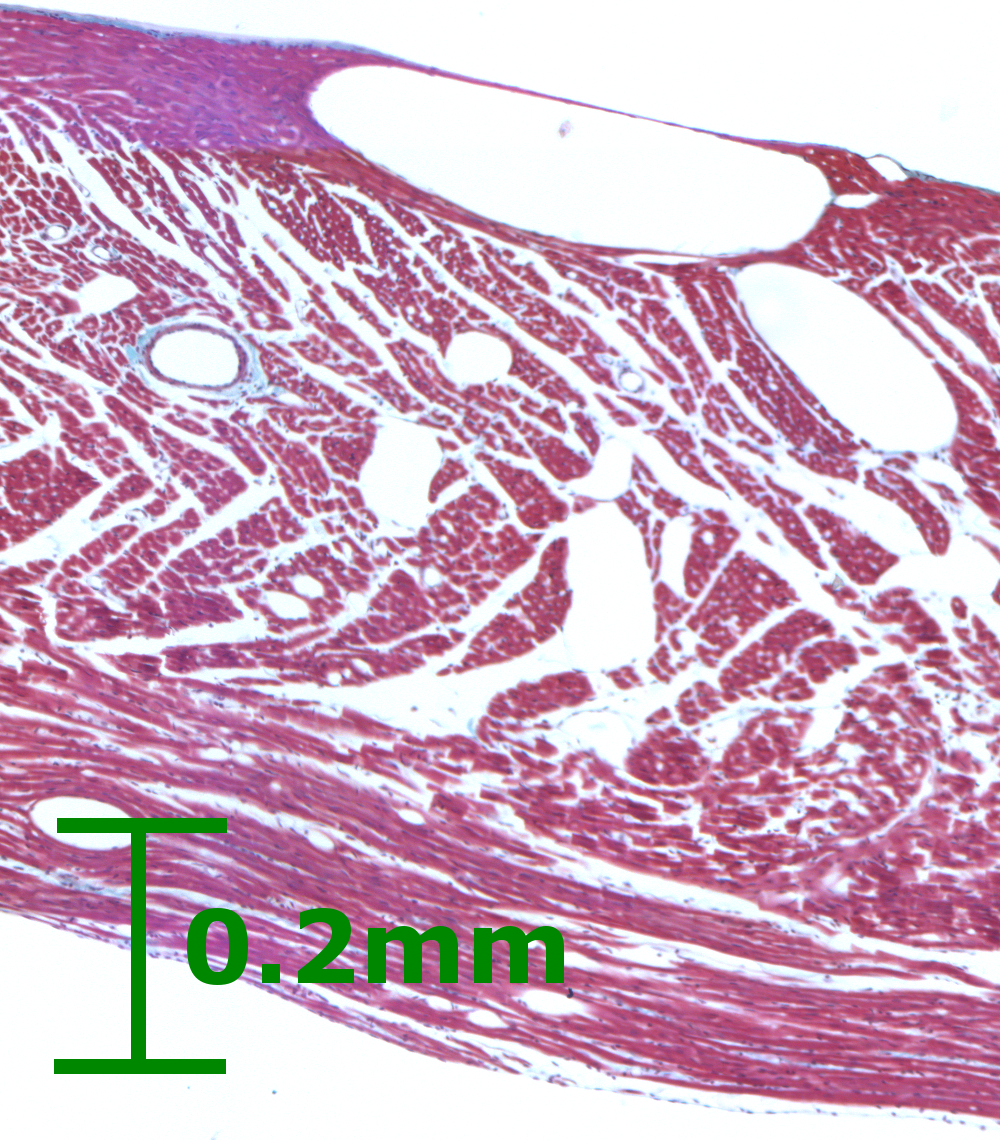
\includegraphics[width=1.7in]{1_introduction/Figs/HiRes_downsamples_1_0582_zoom}}
    \subfloat[]{\includegraphics[width=1.7in]{1_introduction/Figs/LoRes_rgb_downsamples_1_0582_zoom}}
    \caption{Figure on starting point, showing dataset images, whole and with zoom}
    \label{fig:synthetic_cross_sections}
  \end{figure}
    
  
% section introduction (end)
